%%%%%%%%%%%%%%%%%%%%%%%%%%%%%%%%%%%%%%%%%%%%%%%%%%%%%%%%%%%%%%%%%%%%%%
%% Copyright (c) 2016 Carsten Wulff Software, Norway
%% %%%%%%%%%%%%%%%%%%%%%%%%%%%%%%%%%%%%%%%%%%%%%%%%%%%%%%%%%%%%%%%%%%%
%% Created       : wulff at 2016-11-5
%% %%%%%%%%%%%%%%%%%%%%%%%%%%%%%%%%%%%%%%%%%%%%%%%%%%%%%%%%%%%%%%%%%%%
%% This program is free software: you can redistribute it and/or modify
%% it under the terms of the GNU General Public License as published by
%% the Free Software Foundation, either version 3 of the License, or
%% (at your option) any later version.
%%
%% This program is distributed in the hope that it will be useful,
%% but WITHOUT ANY WARRANTY; without even the implied warranty of
%% MERCHANTABILITY or FITNESS FOR A PARTICULAR PURPOSE.  See the
%% GNU General Public License for more details.
%%
%% You should have received a copy of the GNU General Public License
%% along with this program.  If not, see <http://www.gnu.org/licenses/>.
%%%%%%%%%%%%%%%%%%%%%%%%%%%%%%%%%%%%%%%%%%%%%%%%%%%%%%%%%%%%%%%%%%%%%%
%\documentclass[final,11pt]{IEEEtran}
\documentclass[crop,border=0pt]{standalone}
\usepackage{times}


%\usepackage{placeins}
\usepackage{upgreek}
\usepackage{amssymb,amsmath}
\usepackage{cite}
\usepackage{verbatim}
\usepackage{listings}
\usepackage{xcolor}
\usepackage{flafter}
\usepackage{booktabs}
\usepackage{url}
\usepackage{ textcomp }

\hyphenation{op-tical net-works semi-conduc-tor}


% -JSON styel

%\definecolor{darkGreen}{rgb}{0,0.2097,0}
%\newcommand{\myfigwidth}{\linewidth}
%\newcommand{\myfigwidtha}{\linewidth}
%\newcommand{\myfigwidthl}{\textwidth}
%\newcommand{\myfigwidthc}{0.6\linewidth}


\newcommand{\myfigwidtha}{3.3in}
\newcommand{\myfigwidthl}{7in}
\newcommand{\myfigwidthc}{2in}
%\newcommand{\myfigwidthe}{3.2in}
%\newcommand{\myfigwidthb}{5in}

\newcommand{\myfigname}{fig_}
\newcommand{\reg}[2]{{\figurename} \ref{#1}(#2)}
\newcommand{\req}[1]{{\figurename} \ref{#1}}
%\newcommand{\myeqname}{eq:}
%\newcommand{\req}[1]{(\ref{\myeqname#1})}

\definecolor{armygreen}{rgb}{0, 0.5, 0}
\newcommand{\missing}[1]{{ #1}}
\newcommand{\edit}[1]{{ #1}}
\newcommand{\secedit}[1]{{ #1}}
\newcommand{\deleted}[1]{{ #1}}
\newcommand{\moved}[1]{{ #1}}

%\newcommand{\missing}[1]{{\color{red} #1}}
%\newcommand{\edit}[1]{{\color{red} #1}}
%\newcommand{\secedit}[1]{{\color{armygreen} #1}}
%\newcommand{\deleted}[1]{{\color{violet} #1}}
%\newcommand{\moved}[1]{{\color{blue} #1}}

\newcommand{\SD}{Sigma-Delta }
\newcommand{\eqn}[1]{
  \begin{math}
    #1
  \end{math}}

\newcommand\JSONnumbervaluestyle{\color{blue}}
\newcommand\JSONstringvaluestyle{\color{red}}



\newif\ifcolonfoundonthisline

\makeatletter

\lstdefinestyle{json}
{
  showstringspaces    = false,
  keywords            = {false,true},
  alsoletter          = 0123456789.,
  morestring          = [s]{"}{"},
  stringstyle         = \ifcolonfoundonthisline\JSONstringvaluestyle\fi,
  MoreSelectCharTable =%
  \lst@DefSaveDef{`:}\colon@json{\processColon@json},
  basicstyle          = \fontsize{7}{7}\ttfamily,
  keywordstyle        = \fontsize{7}{7}\ttfamily\bfseries,
}

% flip the switch if a colon is found in Pmode
\newcommand\processColon@json{%
  \colon@json%
  \ifnum\lst@mode=\lst@Pmode%
  \global\colonfoundonthislinetrue%
  \fi
}

\lst@AddToHook{Output}{%
  \ifcolonfoundonthisline%
  \ifnum\lst@mode=\lst@Pmode%
  \def\lst@thestyle{\JSONnumbervaluestyle}%
  \fi
  \fi
  % override by keyword style if a keyword is detected!
  \lsthk@DetectKeywords%
}

% reset the switch at the end of line
\lst@AddToHook{EOL}%
{\global\colonfoundonthislinefalse}

\makeatother

% \lstset{  basicstyle=\tiny}

% \lstset{
% basicstyle=\fontsize{11}{13}\selectfont\ttfamily
% }


\lstset{language=Java}




%\usepackage[paperwidth=\maxdimen,paperheight=\maxdimen]{geometry}


\usepackage{tikz,pgfplots}
\usepackage{ifthen}
\usepackage{calc}
\usetikzlibrary{patterns}
%\usepackage[tightpage,active]{preview}
\usetikzlibrary{circuits.logic.US}
\usetikzlibrary{circuits.ee.IEC}
\usepgflibrary{shapes.arrows}
\usepgflibrary{arrows}
\usepackage{circuitikz}


% circuitikz draws bipole outlines (resistors, diodes, capacitors) at
% bipoles/thickness times the ambient line width, and the default is 2.
% That makes a circuitikz resistor visibly heavier than the wire it sits
% on, and heavier than the hand rolled zig-zag in ckt_lib.tex. One is the
% house width: everything is drawn at the environment's own thickness.
% Arrow tips: one filled tip everywhere, set through the '>' knob so a
% figure only ever writes ->, <- or <->. Latex (from arrows.meta)
% scales with the line width, so it stays in proportion if a drawing
% is ever set thicker or thinner than the house 'thick'.
\usetikzlibrary{arrows.meta}
\tikzset{>={Latex}}

\ctikzset{bipoles/thickness=1}
\ctikzset{tripoles/mos style/arrows}
\ctikzset{tripoles/pmos style/emptycircle}
%\PreviewEnvironment{circuitikz}
\pagestyle{empty}


\tikzstyle{cicfill}=[minimum size=1.4em]
\tikzstyle{stuff_fill}=[rectangle,fill=white,minimum size=1.4em]

\newcommand{\grayOne}{0.3 }
\newcommand{\grayTwo}{0.15 }
\newcommand{\grayThree}{0.26 }
\newcommand{\grayFour}{0.41 }
\newcommand{\grayFive}{0.61 }
\newcommand{\graySix}{0.85 }

%- Gray tone
%\definecolor{active}{rgb}{\graySix,\graySix,\graySix}
%\definecolor{poly}{rgb}{\grayFive,\grayFive,\grayFive}
%\definecolor{contact}{rgb}{\graySix,\graySix,\graySix}
%\definecolor{mOne}{rgb}{\grayFour,\grayFour,\grayFour}
%\definecolor{mTwo}{rgb}{\graySix,\graySix,\graySix}
%\definecolor{mThree}{rgb}{\grayThree,\grayThree,\grayThree}
%\definecolor{mFour}{rgb}{\grayTwo,\grayTwo,\grayTwo}

\definecolor{grey}{rgb}{1,1,1}
\definecolor{lightgrey}{rgb}{\grayFour,\grayFour,\grayFour}
\definecolor{active}{rgb}{0.4,1,0.6}
\definecolor{poly}{rgb}{1.0,0.5,0.5}
\definecolor{cut}{rgb}{0.91,0.91,0}
\definecolor{mOne}{rgb}{0.36,0.36,1}
\definecolor{mTwo}{rgb}{0.655,0.655,0}
\definecolor{mThree}{rgb}{0.3,1,1}
\definecolor{mFour}{rgb}{0,0.2097,0}
\begin{document}


% The configuration coordinate diagram of a trap: why capture is
% thermally activated.
%
% The horizontal axis is a lattice coordinate Q, the length of the
% bonds around the defect. The blue parabola is the total energy with
% the electron in the channel and the trap empty; the red one with
% the electron in the trap, where the atoms have moved to make room
% for it. Straight up at fixed Q costs energy the electron does not
% have. It has to wait until a thermal fluctuation of the lattice
% reaches the crossing, where the two states have the same energy and
% the hop is free. That wait is exp(E_B/kT): an Arrhenius law, which
% is what the GR06 trap measures (226 meV).
%
% Parabolas: A = 0.55 (Q-1.5)^2 + 0.5, B = 0.55 (Q-4.3)^2 + 0.2,
% crossing at Q = 2.80, E = 1.43.

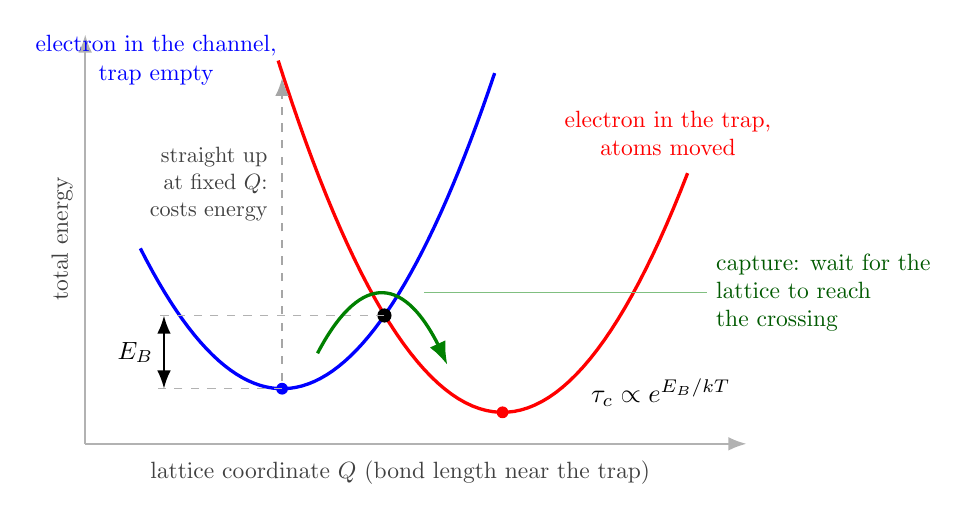
\begin{tikzpicture}[thick]

  % axes
  \draw[gray!60, ->] (-1.0,-0.2) -- (7.4,-0.2);
  \draw[gray!60, ->] (-1.0,-0.2) -- (-1.0,5.0);
  \node[gray!50!black, anchor=north, scale=0.85] at (3.0,-0.3)
    {lattice coordinate $Q$ (bond length near the trap)};
  \node[gray!50!black, anchor=south, rotate=90, scale=0.85] at (-1.05,2.4) {total energy};

  % electron in the channel, trap empty
  \draw[blue, very thick] plot[domain=-0.3:4.2, samples=60] (\x, {0.55*(\x-1.5)^2 + 0.5});
  \node[blue, anchor=south, scale=0.85, align=center] at (-0.1,4.25)
    {electron in the channel,\\trap empty};

  % electron in the trap, lattice relaxed
  \draw[red, very thick] plot[domain=1.45:6.65, samples=60] (\x, {0.55*(\x-4.3)^2 + 0.2});
  \node[red, anchor=south, scale=0.85, align=center] at (6.4,3.35)
    {electron in the trap,\\atoms moved};

  % minima and the crossing
  \fill[blue] (1.5,0.5) circle (0.075);
  \fill[red] (4.3,0.2) circle (0.075);
  \fill[black] (2.80,1.43) circle (0.09);

  % the barrier, measured off to the left
  \draw[gray!60, thin, dashed] (1.5,0.5) -- (-0.15,0.5);
  \draw[gray!60, thin, dashed] (2.80,1.43) -- (-0.15,1.43);
  \draw[<->] (0.0,0.5) -- (0.0,1.43);
  \node[anchor=east, scale=0.9] at (-0.02,0.96) {$E_B$};

  % straight up at fixed Q
  \draw[gray!70, ->, dashed] (1.5,0.6) -- (1.5,4.45);
  \node[gray!50!black, anchor=east, scale=0.8, align=right] at (1.42,3.1)
    {straight up\\at fixed $Q$:\\costs energy};

  % capture over the crossing
  \draw[armygreen, very thick, ->] (1.95,0.95) .. controls (2.5,2.0) and (3.1,2.0) .. (3.6,0.8);
  \draw[armygreen!50, thin] (3.3,1.72) -- (6.9,1.72);
  \node[armygreen!70!black, anchor=west, scale=0.85, align=left] at (6.9,1.72)
    {capture: wait for the\\lattice to reach\\the crossing};
  \node[anchor=west, scale=0.95] at (5.3,0.45) {$\tau_c \propto e^{E_B/kT}$};

\end{tikzpicture}
\end{document}
